\chapter{The Real Numbers: Completing the Line}

\section{The Crisis of Incompleteness}

\begin{intuition}
We have constructed the rationals $\mathbb{Q}$, and they seem to fill the number line. Between any two rationals, there is another rational. They are \textit{dense}.

But the ancient Greeks discovered a terrifying secret: $\mathbb{Q}$ has holes.

Consider the length of the diagonal of a unit square. By Pythagoras, it is a number $x$ such that $x^2 = 2$.
Does such a number exist in $\mathbb{Q}$?
\end{intuition}

\begin{theorem}[Irrationality of $\sqrt{2}$]\index{irrational numbers}\index{square root of 2@$\sqrt{2}$!irrationality}\index{proof by contradiction}
There is no rational number $q \in \mathbb{Q}$ such that $q^2 = 2$.
\end{theorem}

\begin{proof}
Suppose, for the sake of contradiction, that $\sqrt{2}$ is rational.
Then $\sqrt{2} = \frac{p}{q}$ for some $p, q \in \mathbb{Z}, q \neq 0$.
We may assume the fraction is in lowest terms, i.e., $\gcd(p, q) = 1$.

Squaring both sides:
\[ 2 = \frac{p^2}{q^2} \implies p^2 = 2q^2 \]
This means $p^2$ is even. Therefore $p$ must be even (since the square of an odd number is odd).
So $p = 2k$ for some integer $k$.

Substitute back:
\[ (2k)^2 = 2q^2 \implies 4k^2 = 2q^2 \implies 2k^2 = q^2 \]
This means $q^2$ is even, so $q$ must be even.

\textbf{Contradiction}: We found that both $p$ and $q$ are even, meaning they share a common factor of 2. But we assumed $\gcd(p, q) = 1$.

Therefore, no such rational number exists.
\end{proof}

\begin{center}
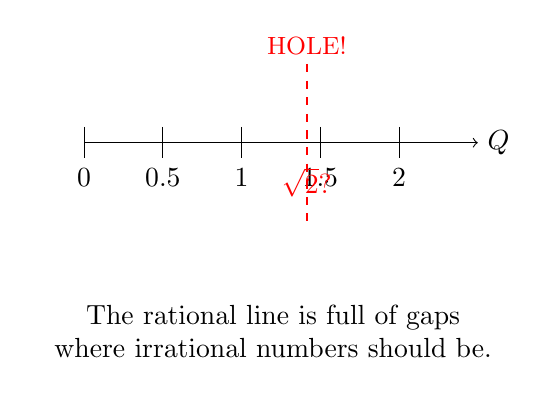
\begin{tikzpicture}[scale=2]
    \draw[->] (0,0) -- (2.5,0);
    \node[right] at (2.5,0) {$\mathbb{Q}$};
    
    \foreach \x in {0, 0.5, 1, 1.5, 2}
        \draw (\x, 0.1) -- (\x, -0.1) node[below] {\x};
        
    \node[red, below] at (1.414, -0.1) {$\sqrt{2}$?};
    \draw[red, thick, dashed] (1.414, 0.5) -- (1.414, -0.5);
    
    \node[above, red] at (1.414, 0.5) {\small HOLE!};
    
    \node[align=center, text width=6cm] at (1.2, -1.2) {The rational line is full of gaps where irrational numbers should be.};
\end{tikzpicture}
\end{center}

\section{Dedekind Cuts: Constructing the Continuum}

How do we fill these gaps? Richard Dedekind (1872) had a brilliant insight: \textbf{Define a real number by the set of all rational numbers smaller than it.}

Instead of trying to grasp the elusive $\sqrt{2}$ directly, we look at its "shadow" on the rational line: all rationals $q$ such that $q^2 < 2$ (or $q < 0$).

\begin{definition}[Dedekind Cut]\index{Dedekind cut}\index{real numbers!Dedekind cuts}\index{cut, Dedekind}
A \textbf{Dedekind cut} is a subset $\alpha \subseteq \mathbb{Q}$ such that:
\begin{enumerate}
    \item \textbf{Non-trivial}: $\alpha \neq \emptyset$ and $\alpha \neq \mathbb{Q}$.
    \item \textbf{Closed downwards}: If $p \in \alpha$ and $q < p$, then $q \in \alpha$.
    \item \textbf{No greatest element}: If $p \in \alpha$, there exists $r \in \alpha$ such that $p < r$.
\end{enumerate}

The set of all Dedekind cuts is denoted by $\mathbb{R}$.
\end{definition}

\begin{intuition}
Think of cutting the rational number line with a pair of scissors. The cut divides $\mathbb{Q}$ into two parts: the left set ($L$) and the right set ($R$).
We identify the real number with the left set $\alpha = L$.

\begin{itemize}
    \item Condition 1 ensures we don't pick "nothing" or "everything".
    \item Condition 2 means $\alpha$ is an initial segment of the line.
    \item Condition 3 is a technical convenience (it avoids ambiguity for rational numbers like "everything strictly less than 1" vs "everything less than or equal to 1"). We choose strict inequality.
\end{itemize}
\end{intuition}

\begin{remark}[Alternative Construction: Cauchy Sequences]
The Dedekind cut approach is not the only way to construct $\mathbb{R}$ from $\mathbb{Q}$. Another classical method uses \textbf{Cauchy sequences}.

\textbf{Cauchy Sequence Approach:}

A sequence $(q_n)$ of rational numbers is \textbf{Cauchy} if for every $\varepsilon \in \mathbb{Q}$ with $\varepsilon > 0$, there exists $N \in \mathbb{N}$ such that for all $m, n \geq N$:
\[|q_m - q_n| < \varepsilon\]

Intuitively, the terms get arbitrarily close to each other. In $\mathbb{Q}$, Cauchy sequences need not converge (e.g., the sequence $1, 1.4, 1.41, 1.414, \ldots$ approximating $\sqrt{2}$ is Cauchy in $\mathbb{Q}$ but has no rational limit).

We define:
\begin{itemize}
    \item Two Cauchy sequences $(p_n)$ and $(q_n)$ are \textbf{equivalent} if $\lim_{n \to \infty} |p_n - q_n| = 0$ (in the sense that for all $\varepsilon > 0$, eventually $|p_n - q_n| < \varepsilon$).
    
    \item A real number is an equivalence class of Cauchy sequences of rationals.
    
    \item $\mathbb{R} := \{\text{Cauchy sequences in } \mathbb{Q}\} / {\sim}$
\end{itemize}

Operations are defined component-wise: $(p_n) + (q_n) := (p_n + q_n)$, etc.

\textbf{Comparison of the Two Constructions:}

\begin{center}
\begin{tabular}{|l|p{5cm}|p{5cm}|}
\hline
\textbf{Aspect} & \textbf{Dedekind Cuts} & \textbf{Cauchy Sequences} \\
\hline
\textbf{Definition} & A set of rationals (an initial segment) & An equivalence class of sequences \\
\hline
\textbf{Intuition} & "All rationals less than $x$" & "Sequences converging to $x$" \\
\hline
\textbf{Order} & Natural: $\alpha < \beta$ iff $\alpha \subsetneq \beta$ & Requires definition via representatives \\
\hline
\textbf{Operations} & Set-theoretic (unions, products of sets) & Component-wise on sequences \\
\hline
\textbf{Pros} & Order structure immediate; completeness easy to prove & Generalizes to abstract metric spaces; dynamic/constructive feel \\
\hline
\textbf{Cons} & Abstract (real number as infinite set); operations technical & Equivalence relation subtle; order less natural \\
\hline
\textbf{Historical} & Dedekind (1872) & Cantor (1872), Méray (1869) \\
\hline
\end{tabular}
\end{center}

\textbf{Are They the Same?}

Yes! Both constructions yield \textit{isomorphic} complete ordered fields. There is a natural bijection:
\begin{itemize}
    \item Given a Dedekind cut $\alpha$, construct a Cauchy sequence $(q_n)$ where $q_n \in \alpha$ approaches the "boundary" of $\alpha$ from below.
    
    \item Given a Cauchy sequence $(q_n)$, define the cut $\alpha = \{r \in \mathbb{Q} : r < q_n \text{ for infinitely many } n\}$.
\end{itemize}

This bijection preserves $+$, $\cdot$, and $<$, making the two constructions mathematically equivalent.

\textbf{Why We Choose Dedekind Cuts Here:}

We use Dedekind cuts because:
\begin{itemize}
    \item Order is immediately transparent (set inclusion)
    \item Completeness (least upper bound property) is straightforward to verify
    \item They fit naturally in our set-theoretic framework built from ZFC
\end{itemize}

However, Cauchy sequences are indispensable in analysis and topology, where metric completeness generalizes beyond $\mathbb{R}$ to arbitrary metric spaces. Both perspectives enrich understanding.
\end{remark}


\begin{example}[Representing Numbers]
\textbf{The Rational 1}:
\[ 1^* = \{q \in \mathbb{Q} : q < 1\} \]
This is a cut representing the real number 1.

\textbf{The Irrational $\sqrt{2}$}:
\[ \sqrt{2}^* = \{q \in \mathbb{Q} : q < 0 \text{ or } q^2 < 2\} \]
This set contains all negative rationals, and positive rationals whose square is less than 2 (e.g., 1, 1.4, 1.41...). It satisfies all conditions of a cut.
\end{example}

\section{Ordering the Reals}

Defining order on Dedekind cuts is elegant: it's just subset inclusion.

\begin{definition}[Order on $\mathbb{R}$]
Let $\alpha, \beta \in \mathbb{R}$. We define:
\[ \alpha \le \beta \iff \alpha \subseteq \beta \]
\end{definition}

\begin{theorem}
$(\mathbb{R}, \le)$ is a total order.
\end{theorem}

\begin{proof}
Reflexivity and transitivity follow immediately from set inclusion properties.
Total ordering (comparability) relies on the property of cuts: if $\alpha \not\subseteq \beta$, there is a rational $p \in \alpha$ such that $p \notin \beta$. Since $\beta$ is closed downwards, this implies $p$ is greater than or equal to every element in $\beta$, essentially meaning $\beta \subset \alpha$ (with minor technical details to fill).
\end{proof}

\section{Arithmetic on $\mathbb{R}$}

\subsection{Addition}

\begin{definition}[Addition]
Let $\alpha, \beta \in \mathbb{R}$. Their sum is defined as the set of all sums of their elements:
\[ \alpha + \beta := \{x + y : x \in \alpha, y \in \beta\} \]
\end{definition}

We must verify that $\alpha + \beta$ is indeed a Dedekind cut (non-empty, closed downwards, no max).
\begin{itemize}
    \item If $x \in \alpha, y \in \beta$, and $z < x+y$, is $z \in \alpha+\beta$? Yes. Let $\delta = (x+y) - z$. Then $(x-\delta/2) \in \alpha$ and $(y-\delta/2) \in \beta$, summing to $z$.
\end{itemize}

\subsection{Multiplication}

Multiplication is trickier due to negative numbers (multiplying two large negative numbers gives a large positive number, not a small one).

\begin{definition}[Multiplication of Positive Reals]
For $\alpha, \beta > 0^*$ (positive cuts), define:
\[ \alpha \cdot \beta = \{p \cdot q : p \in \alpha, p > 0, q \in \beta, q > 0\} \cup \{r \in \mathbb{Q} : r \leq 0\} \]

\textbf{Interpretation}: We take all products of positive elements from $\alpha$ and $\beta$, and include all non-positive rationals to ensure the result is closed downwards.
\end{definition}

\begin{theorem}
If $\alpha, \beta > 0^*$, then $\alpha \cdot \beta$ is a Dedekind cut.
\end{theorem}

\begin{proof}[Proof Sketch]
We verify the three conditions:

\textbf{(1) Non-trivial}: $\alpha \cdot \beta \neq \emptyset$ (contains $0$ and negative rationals). Also $\alpha \cdot \beta \neq \mathbb{Q}$ because if $p \in \alpha$ is positive and bounded, and $q \in \beta$ is positive and bounded, then any rational larger than all possible products $pq$ is not in $\alpha \cdot \beta$.

\textbf{(2) Closed downwards}: If $r \in \alpha \cdot \beta$ and $s < r$:
\begin{itemize}
    \item If $r \leq 0$, then $s < 0$, so $s \in \alpha \cdot \beta$ by definition.
    \item If $r > 0$, then $r = p \cdot q$ for some $p \in \alpha, p > 0, q \in \beta, q > 0$. 
    
    Since $s < r = pq$ and both $p, q > 0$, we can find $p' \in \alpha$ with $p' < p$ close enough that $p' \cdot q < s < p \cdot q$. 
    
    Then $s$ can be written as a product of positive elements from the cuts (or is $\leq 0$), so $s \in \alpha \cdot \beta$.
\end{itemize}

\textbf{(3) No maximum}: If $r \in \alpha \cdot \beta$ and $r > 0$, say $r = p \cdot q$ with $p \in \alpha, q \in \beta$. Since $\alpha$ has no maximum, there exists $p' \in \alpha$ with $p' > p$. Then $p' \cdot q > r$ and $p' \cdot q \in \alpha \cdot \beta$. $\checkmark$
\end{proof}

\begin{definition}[Multiplication for All Reals]
For arbitrary $\alpha, \beta \in \mathbb{R}$, define multiplication using sign rules:

\begin{enumerate}
    \item If $\alpha, \beta > 0^*$: Use the definition above
    \item If $\alpha > 0^*, \beta < 0^*$: Define $\alpha \cdot \beta = -(\alpha \cdot (-\beta))$
    \item If $\alpha < 0^*, \beta > 0^*$: Define $\alpha \cdot \beta = -((-\alpha) \cdot \beta)$
    \item If $\alpha, \beta < 0^*$: Define $\alpha \cdot \beta = (-\alpha) \cdot (-\beta)$
    \item If $\alpha = 0^*$ or $\beta = 0^*$: Define $\alpha \cdot \beta = 0^*$
\end{enumerate}

where $-\alpha = \{q \in \mathbb{Q} : \exists r \notin \alpha, q < -r\}$ (additive inverse).
\end{definition}

\begin{theorem}[Field Properties]
$(\mathbb{R}, +, \cdot)$ forms a field:
\begin{itemize}
    \item Addition and multiplication are associative and commutative
    \item Distributive law: $\alpha(\beta + \gamma) = \alpha\beta + \alpha\gamma$
    \item Additive identity $0^*$ and multiplicative identity $1^*$
    \item Every element has an additive inverse
    \item Every non-zero element has a multiplicative inverse
\end{itemize}
\end{theorem}

\begin{proof}[Verification of Field Axioms for $\mathbb{R}$]
We verify the key axioms. The others follow similarly.

\textbf{(1) Commutativity of Addition}: $\alpha + \beta = \beta + \alpha$

For cuts $\alpha$ and $\beta$, by definition:
\[\alpha + \beta = \{r + s : r \in \alpha, s \in \beta\}\]
\[\beta + \alpha = \{s + r : s \in \beta, r \in \alpha\}\]

Since addition in $\mathbb{Q}$ is commutative ($r + s = s + r$), these sets are equal. $\checkmark$

\textbf{(2) Associativity of Addition}: $(\alpha + \beta) + \gamma = \alpha + (\beta + \gamma)$

Both sides equal $\{r + s + t : r \in \alpha, s \in \beta, t \in \gamma\}$ by associativity in $\mathbb{Q}$. $\checkmark$

\textbf{(3) Additive Identity}: $\alpha + \mathbf{0} = \alpha$ where $\mathbf{0} = \{r \in \mathbb{Q} : r < 0\}$

By definition:
\[\alpha + \mathbf{0} = \{r + s : r \in \alpha, s \in \mathbf{0}\}\]

For any $a \in \alpha$, pick $s < 0$ in $\mathbf{0}$ such that $a + s \in \alpha$ (possible since $\alpha$ has no greatest element). Conversely, if $a + s \in \alpha + \mathbf{0}$ with $s < 0$, then $a \in \alpha$. Thus $\alpha + \mathbf{0} = \alpha$. $\checkmark$

\textbf{(4) Commutativity of Multiplication}: $\alpha \cdot \beta = \beta \cdot \alpha$

For positive cuts, by definition (assuming $\alpha, \beta > \mathbf{0}$):
\[\alpha \cdot \beta = \{rs : r \in \alpha, s \in \beta, r > 0, s > 0\} \cup \{q \in \mathbb{Q} : q \leq 0\}\]

Since $rs = sr$ in $\mathbb{Q}$, we have $\alpha \cdot \beta = \beta \cdot \alpha$. $\checkmark$

For negative cuts, the sign rules ensure commutativity is preserved. $\checkmark$

\textbf{(5) Associativity of Multiplication}: $(\alpha \cdot \beta) \cdot \gamma = \alpha \cdot (\beta \cdot \gamma)$

For positive cuts, both sides equal:
\[\{rst : r \in \alpha, s \in \beta, t \in \gamma, r, s, t > 0\} \cup \{q \in \mathbb{Q} : q \leq 0\}\]

by associativity in $\mathbb{Q}$. $\checkmark$

\textbf{(6) Multiplicative Identity}: $\alpha \cdot \mathbf{1} = \alpha$ where $\mathbf{1} = \{r \in \mathbb{Q} : r < 1\}$

For $\alpha > \mathbf{0}$:
\[\alpha \cdot \mathbf{1} = \{rs : r \in \alpha, s \in \mathbf{1}, r > 0, s > 0\} \cup \{q \in \mathbb{Q} : q \leq 0\}\]

For any $a \in \alpha$ with $a > 0$, pick $s \in \mathbf{1}$ with $s > 0$ close to $1$ such that $as \in \alpha$ (using density of $\mathbb{Q}$). Conversely, if $as \in \alpha \cdot \mathbf{1}$ with $s < 1$, then $a \in \alpha$ (since $as < a$ and $\alpha$ is downward closed). Thus $\alpha \cdot \mathbf{1} = \alpha$. $\checkmark$

\textbf{(7) Distributivity}: $\alpha \cdot (\beta + \gamma) = \alpha \cdot \beta + \alpha \cdot \gamma$

This is the most involved axiom. We verify for positive cuts $\alpha, \beta, \gamma > \mathbf{0}$.

\textbf{Left-hand side}:
\[\beta + \gamma = \{s + t : s \in \beta, t \in \gamma\}\]
\[\alpha \cdot (\beta + \gamma) = \{r(s + t) : r \in \alpha, s \in \beta, t \in \gamma, r, s, t > 0\} \cup \{q : q \leq 0\}\]

\textbf{Right-hand side}:
\[\alpha \cdot \beta = \{rs : r \in \alpha, s \in \beta, r > 0, s > 0\} \cup \{q : q \leq 0\}\]
\[\alpha \cdot \gamma = \{rt : r \in \alpha, t \in \gamma, r > 0, t > 0\} \cup \{q : q \leq 0\}\]
\[\alpha \cdot \beta + \alpha \cdot \gamma = \{rs + rt : r \in \alpha, s \in \beta, t \in \gamma, r, s, t > 0\} \cup \{q : q \leq 0\}\]

By distributivity in $\mathbb{Q}$: $r(s + t) = rs + rt$, so both sides are equal. $\checkmark$

For mixed signs (some cuts negative), the sign rules ensure distributivity holds by reducing to the positive case with appropriate sign adjustments. The verification is case-by-case but follows the same logic. $\checkmark$

Therefore $\mathbb{R}$ satisfies all field axioms.
\end{proof}

\begin{keyidea}
\textbf{Why this construction works}:

We've built $\mathbb{R}$ from $\mathbb{Q}$ using only set theory. The operations $+$ and $\cdot$ on cuts are defined so that:
\begin{itemize}
    \item They extend the operations on $\mathbb{Q}$ (rational cuts behave like rationals)
    \item They preserve algebraic properties (field axioms)
    \item They respect order ($\alpha < \beta \implies \alpha + \gamma < \beta + \gamma$)
    \item They fill the gaps (completeness property)
\end{itemize}

The price we pay is abstraction: real numbers are now \textit{infinite sets} of rationals!

But this gives us rigorous foundations for calculus.
\end{keyidea}

\section{Absolute Value and Distance}

To talk about "closeness" and "limits" in the next chapter, we need a way to measure size and distance.

\begin{definition}[Absolute Value]
For $x \in \mathbb{R}$, the \textbf{absolute value} $|x|$ is defined as:
\[ |x| = \begin{cases} x & \text{if } x \geq 0 \\ -x & \text{if } x < 0 \end{cases} \]
\end{definition}

\begin{theorem}[Properties of Absolute Value]
For all $x, y \in \mathbb{R}$:
\begin{enumerate}
    \item \textbf{Non-negativity}: $|x| \geq 0$, and $|x| = 0 \iff x = 0$.
    \item \textbf{Multiplicativity}: $|xy| = |x||y|$.
    \item \textbf{Triangle Inequality}: $|x + y| \leq |x| + |y|$.
\end{enumerate}
\end{theorem}

\begin{proof}[Proof of Triangle Inequality]
Notice that $-|x| \leq x \leq |x|$ and $-|y| \leq y \leq |y|$.
Adding these inequalities:
\[ -(|x| + |y|) \leq x + y \leq |x| + |y| \]
This is equivalent to $|x + y| \leq |x| + |y|$.
\end{proof}

\begin{definition}[Distance]
The \textbf{distance} between two real numbers $x$ and $y$ is defined as:
\[ d(x, y) := |x - y| \]
\end{definition}

\begin{remark}
This distance function $d$ makes $\mathbb{R}$ into a \textbf{metric space}. It satisfies:
\begin{itemize}
    \item $d(x, y) \geq 0$
    \item $d(x, y) = d(y, x)$ (Symmetry)
    \item $d(x, z) \leq d(x, y) + d(y, z)$ (Triangle Inequality for distance)
\end{itemize}
This metric is the foundation of all analysis on the real line.
\end{remark}

\section{Topology of the Real Line}

The structure of "open" and "closed" sets on $\mathbb{R}$ is crucial for rigorously defining continuity, limits, and convergence. While a full course on topology is beyond our scope, we establish the essential definitions needed for analysis.

\begin{definition}[Open Intervals]
For $a, b \in \mathbb{R}$ with $a < b$, the \textbf{open interval} is:
\[(a, b) := \{x \in \mathbb{R} : a < x < b\}\]

We also define unbounded open intervals:
\[(a, \infty) := \{x \in \mathbb{R} : x > a\}, \quad (-\infty, b) := \{x \in \mathbb{R} : x < b\}, \quad (-\infty, \infty) := \mathbb{R}\]
\end{definition}

\begin{definition}[Open Sets]
A subset $U \subseteq \mathbb{R}$ is called \textbf{open} if:

For every $x \in U$, there exists $\varepsilon > 0$ such that $(x - \varepsilon, x + \varepsilon) \subseteq U$.

Intuitively: every point in $U$ is surrounded by a "buffer zone" also contained in $U$.
\end{definition}

\begin{example}
\begin{itemize}
    \item $(0, 1)$ is open: for any $x \in (0, 1)$, take $\varepsilon = \min(x, 1-x)/2$ to get $(x - \varepsilon, x + \varepsilon) \subseteq (0, 1)$.
    
    \item $[0, 1]$ is \textit{not} open: the point $0 \in [0, 1]$, but for any $\varepsilon > 0$, the interval $(0 - \varepsilon, 0 + \varepsilon) = (-\varepsilon, \varepsilon)$ contains $-\varepsilon/2 \notin [0, 1]$.
    
    \item $\mathbb{R}$ is open (vacuously satisfied for all points).
    
    \item $\emptyset$ is open (vacuously satisfied, no points to check).
\end{itemize}
\end{example}

\begin{theorem}[Properties of Open Sets]
The collection of open sets in $\mathbb{R}$ satisfies:
\begin{enumerate}
    \item $\emptyset$ and $\mathbb{R}$ are open.
    \item The union of any collection of open sets is open.
    \item The intersection of finitely many open sets is open.
\end{enumerate}
\end{theorem}

\begin{proof}[Proof Sketch]
\textbf{(1)} Already verified above.

\textbf{(2)} If $\{U_i : i \in I\}$ is a collection of open sets, let $U = \bigcup_{i \in I} U_i$.

For any $x \in U$, there exists $i \in I$ such that $x \in U_i$. Since $U_i$ is open, there exists $\varepsilon > 0$ such that $(x - \varepsilon, x + \varepsilon) \subseteq U_i \subseteq U$. $\checkmark$

\textbf{(3)} Let $U_1, \ldots, U_n$ be open sets, and let $U = \bigcap_{j=1}^n U_j$.

For any $x \in U$, we have $x \in U_j$ for all $j$. For each $j$, there exists $\varepsilon_j > 0$ such that $(x - \varepsilon_j, x + \varepsilon_j) \subseteq U_j$.

Let $\varepsilon = \min(\varepsilon_1, \ldots, \varepsilon_n) > 0$. Then $(x - \varepsilon, x + \varepsilon) \subseteq U_j$ for all $j$, so $(x - \varepsilon, x + \varepsilon) \subseteq U$. $\checkmark$
\end{proof}

\begin{warning}
\textbf{Infinite intersections of open sets need not be open!}

Consider $U_n = \left(-\frac{1}{n}, \frac{1}{n}\right)$ for $n \in \mathbb{N}$. Each $U_n$ is open.

But:
\[\bigcap_{n=1}^\infty U_n = \{0\}\]

which is \textit{not} open (no $\varepsilon$-neighborhood around $0$ fits inside $\{0\}$).
\end{warning}

\begin{definition}[Closed Sets]
A subset $F \subseteq \mathbb{R}$ is called \textbf{closed} if its complement $\mathbb{R} \setminus F$ is open.
\end{definition}

\begin{example}
\begin{itemize}
    \item $[0, 1]$ is closed: $\mathbb{R} \setminus [0, 1] = (-\infty, 0) \cup (1, \infty)$ is open (union of open sets).
    
    \item $(0, 1)$ is \textit{not} closed: $\mathbb{R} \setminus (0, 1) = (-\infty, 0] \cup [1, \infty)$ is not open (contains $0$ and $1$ without neighborhoods).
    
    \item $\mathbb{R}$ is both open and closed.
    
    \item $\emptyset$ is both open and closed.
    
    \item $[0, 1)$ is \textit{neither} open nor closed.
\end{itemize}
\end{example}

\begin{definition}[Topology on $\mathbb{R}$]
The collection $\mathcal{T}$ of all open subsets of $\mathbb{R}$ is called the \textbf{standard topology} on $\mathbb{R}$ (or the \textbf{Euclidean topology}).

The pair $(\mathbb{R}, \mathcal{T})$ is a \textbf{topological space}.
\end{definition}

\begin{remark}
This topology is induced by the metric $d(x, y) = |x - y|$. In general, any metric space has a natural topology where open sets are unions of open balls.

All the key notions of calculus---continuity, limits, compactness---can be defined using only open sets, making topology the natural language of analysis.
\end{remark}

\section{The Completeness Axiom}

This is the crowning jewel of the real numbers. The "holes" are gone.

\begin{definition}[Bounds and Suprema/Infima]
Let $S \subseteq \mathbb{R}$.
\begin{itemize}
    \item $M \in \mathbb{R}$ is an \textbf{upper bound} for $S$ if $s \leq M$ for all $s \in S$.
    \item $M$ is the \textbf{supremum} (least upper bound), denoted $\sup S$, if it is an upper bound and $M \leq K$ for any other upper bound $K$.
    \item $m \in \mathbb{R}$ is a \textbf{lower bound} for $S$ if $s \geq m$ for all $s \in S$.
    \item $m$ is the \textbf{infimum} (greatest lower bound), denoted $\inf S$, if it is a lower bound and $m \geq k$ for any other lower bound $k$.
\end{itemize}
\end{definition}

\begin{theorem}[Least Upper Bound Property]\index{least upper bound property}\index{supremum}\index{completeness!of real numbers}\index{LUB property}
Every non-empty subset of $\mathbb{R}$ that has an upper bound has a supremum in $\mathbb{R}$.
\end{theorem}

\begin{intuition}
In $\mathbb{Q}$, the set $S = \{q \in \mathbb{Q} : q^2 < 2\}$ is bounded above (e.g., by 2), but has no least upper bound \textit{in $\mathbb{Q}$} (because $\sqrt{2} \notin \mathbb{Q}$).
In $\mathbb{R}$, the supremum is exactly the cut for $\sqrt{2}$. The "hole" has been filled by the cut itself.
\end{intuition}

\begin{proof}[Proof Sketch]
Let $\mathcal{A} \subseteq \mathbb{R}$ be a non-empty set of cuts bounded above.
Consider the union of all these cuts:
\[ \gamma = \bigcup_{\alpha \in \mathcal{A}} \alpha \]
Remarkably, $\gamma$ itself is a Dedekind cut!
\begin{enumerate}
    \item Since each $\alpha$ is a subset of rationals, $\gamma \subseteq \mathbb{Q}$.
    \item $\gamma$ is closed downwards because each $\alpha$ is.
    \item $\gamma$ is clearly $\ge \alpha$ for all $\alpha \in \mathcal{A}$ (superset relation).
    \item $\gamma$ is the \textit{least} such bound.
\end{enumerate}
Thus, $\sup \mathcal{A} = \bigcup \mathcal{A}$. The supremum is literally the union of the sets.
\end{proof}

\section{Density of Rationals}

Even though $\mathbb{Q}$ is incomplete, it is \textbf{dense} in $\mathbb{R}$.

\begin{theorem}[Density of $\mathbb{Q}$]\index{density of rationals}\index{rational numbers!density}\index{Q@$\mathbb{Q}$!density in R@$\mathbb{R}$}
For any two real numbers $x < y$, there exists a rational number $q$ such that $x < q < y$.
\end{theorem}

\begin{proof}
Let $x, y$ be Dedekind cuts with $x \subsetneq y$.
By definition of set inclusion, there exists a rational $q \in y$ such that $q \notin x$.
Since $x$ is closed downwards, $q \notin x$ implies $q$ is greater than or equal to every element in $x$.
Strictly speaking, we need slightly more care to find a $q$ strictly "between", but the nature of cuts provides this rational witness immediately.
\end{proof}

\section{Looking Forward}

We have built the \textbf{complete ordered field} $\mathbb{R}$.
\begin{itemize}
    \item It allows us to solve equations like $x^2 = 2$.
    \item It has no gaps ($\sup$ always exists).
\end{itemize}

However, we defined reals as \textit{sets} of rationals. In calculus, we often think of reals as limits of sequences (e.g., $3, 3.1, 3.14, 3.141, \dots$).
In the next chapter, \textbf{Sequences and Convergence}, we will bridge these two views and rigorously define limits.
